\section{Скриншоты}

\subsection{Первая программа}
\begin{figure}[H]
  \centering
  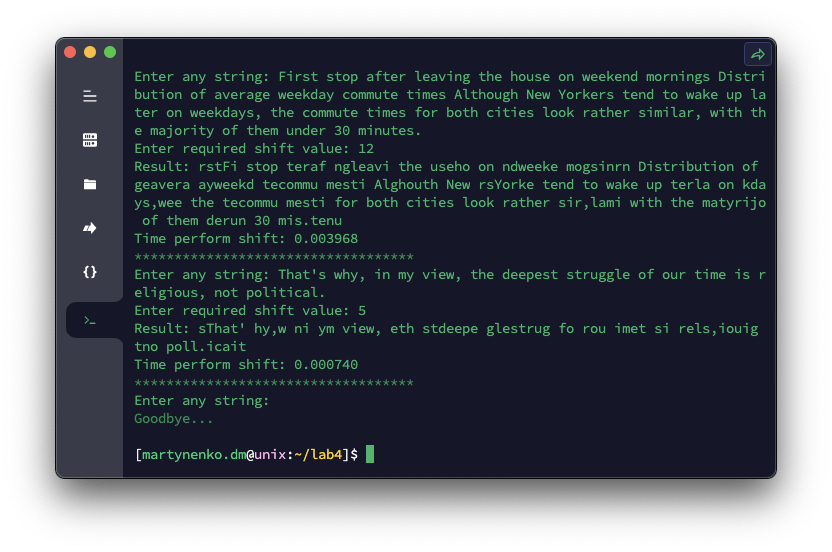
\includegraphics[width=0.80\textwidth]{screenshot_default}
  \caption{Работа программы с использованием библиотечных функций.}
\end{figure}

\subsection{Вторая программа}
\begin{figure}[H]
  \centering
  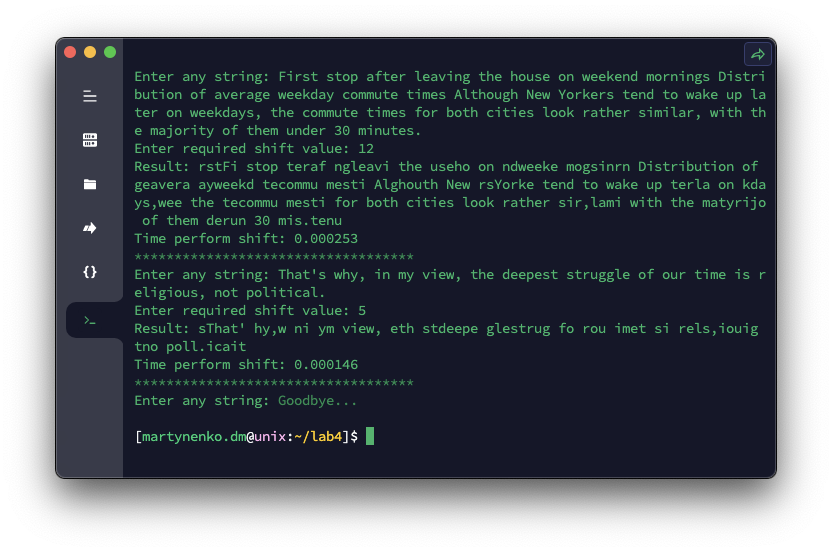
\includegraphics[width=0.80\textwidth]{screenshot_custom}
  \caption{Работа программы без использования библиотечных функций.}
\end{figure}

\subsection{Использование памяти}
\begin{figure}[H]
  \centering
  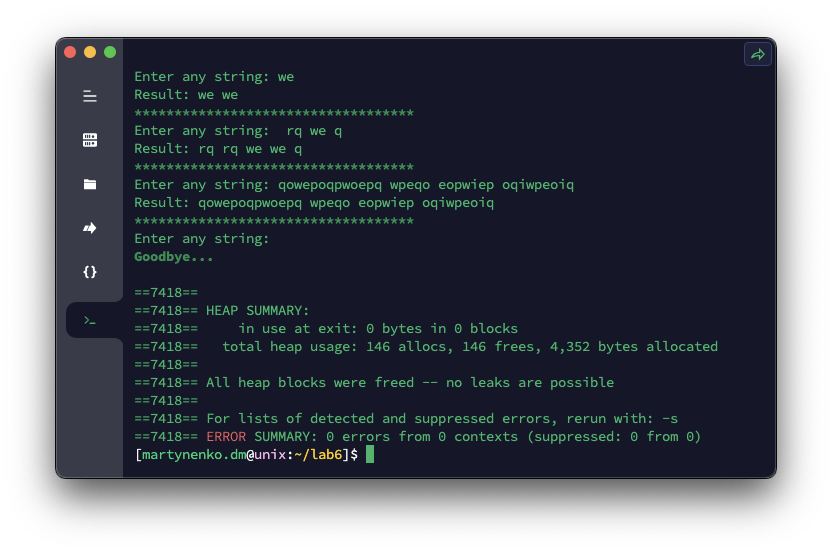
\includegraphics[width=0.80\textwidth]{screenshot_valgrind}
  \caption{Успешная проверка использования памяти при помощи valgrind.}
\end{figure}
